\documentclass{article}
\usepackage{tikz}\usetikzlibrary{backgrounds}
\begin{document}
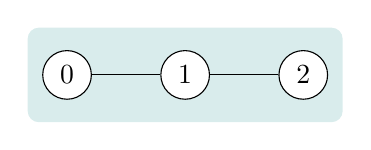
\begin{tikzpicture}
\foreach \x in {0,1,2}{\node[draw,circle,fill=white] (n\x) at (\x*1.5,0){\x};}
\draw (n0)--(n1)--(n2);
\begin{scope}[on background layer]
\fill[teal!15,rounded corners] (-.5,-.6) rectangle (3.5,.6);
\end{scope}
\end{tikzpicture}
\end{document}
